% Created 2021-01-08 Fri 11:05
% Intended LaTeX compiler: pdflatex
\documentclass[a4paper,11pt,twoside]{article}
\usepackage[utf8]{inputenc}
\usepackage[T1]{fontenc}
\usepackage{graphicx}
\usepackage{grffile}
\usepackage{longtable}
\usepackage{wrapfig}
\usepackage{rotating}
\usepackage[normalem]{ulem}
\usepackage{amsmath}
\usepackage{textcomp}
\usepackage{amssymb}
\usepackage{capt-of}
\usepackage{hyperref}
\usepackage{minted}
\IfFileExists{./resources/style.sty}{\usepackage{./resources/style}}{}
\IfFileExists{./resources/referencing.sty}{\usepackage{./resources/referencing}}{}
\addbibresource{../resources/references.bib}
\usepackage[mode=buildnew]{standalone}
\usepackage{tikz}
\usetikzlibrary{decorations.fractals}
\usetikzlibrary{lindenmayersystems}
\author{Ryan Greenup}
\date{\today}
\title{RankNet Investigatoin}
\hypersetup{
 pdfauthor={Ryan Greenup},
 pdftitle={RankNet Investigatoin},
 pdfkeywords={},
 pdfsubject={},
 pdfcreator={Emacs 27.1 (Org mode 9.4)}, 
 pdflang={English}}
\begin{document}

\maketitle
\tableofcontents

\# \#+TODO: TODO IN-PROGRESS WAITING DONE
 \newpage 
\section{Text and References}
\label{sec:org38d1ca3}
Fractals are complex shapes that often occur from natural processes, in this
report we hope to investigate the emergence of patterns and complex structures
from natural phenomena. We begin with an investigation into fractals and the
concept of dimension and then discuss links between fractal patterns and natural
processes.

This is a Reference \cite{tuGraphBasedSemiSupervisedNearestNeighbor2016a} and another \cite{nicodemiIntroductionAbstractAlgebra2007a} and yet another \cite{christopherburgesRankNetLambdaRankLambdaMART2010}.

\section{Fractals}
\label{sec:org6f6c5b5}
Images are shown in figure \ref{imtest}.

\begin{figure}[htbp]
\centering
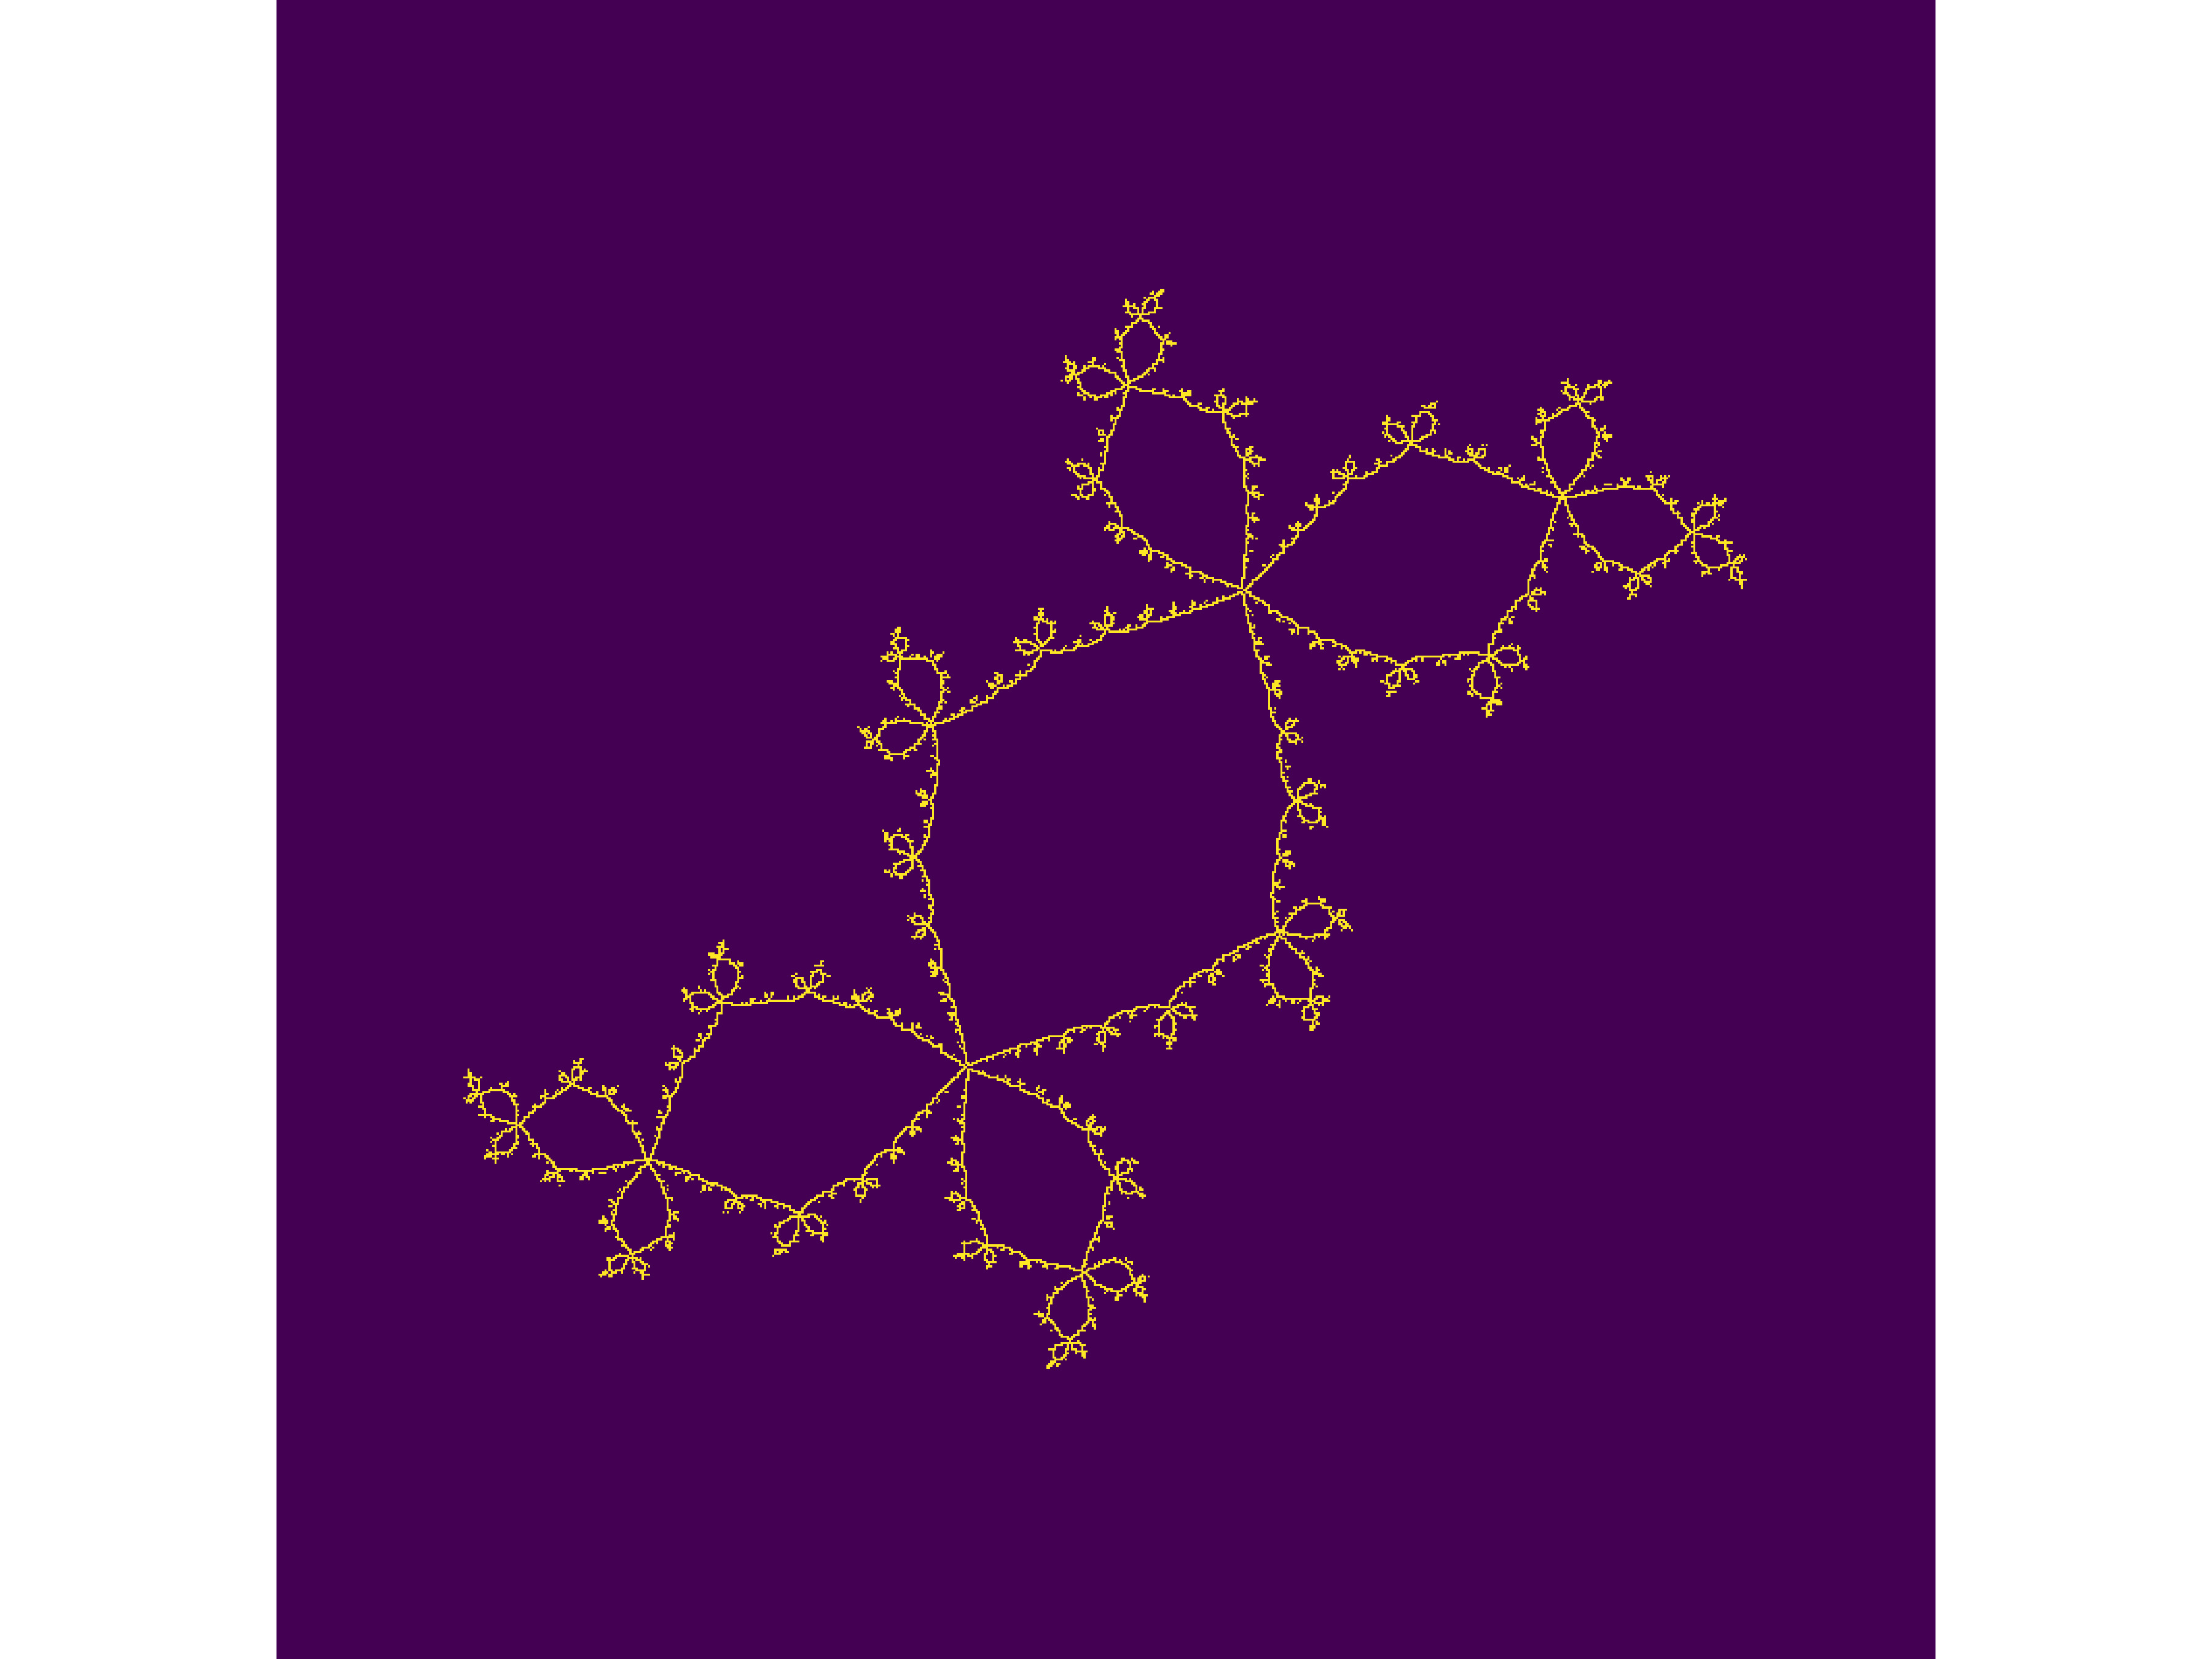
\includegraphics[width=0.5\textwidth]{media/outline-rabbit.png}
\caption{\label{imtest}This is a test image showing the outline of a Julia set}
\end{figure}
\end{document}
